\documentclass[pdf, aspectratio=169, 12pt]{beamer}
\usepackage[]{hyperref, graphicx, siunitx, lmodern, tikz, booktabs, physics, multicol}
\usepackage[mode=buildnew]{standalone}
\usepackage{pdfpc-commands}
\usepackage{pgfplots}
\pgfplotsset{compat=1.16}

\usetheme[sols]{Python}

\graphicspath{ {Images/} }

\sisetup{per-mode=symbol}
\usetikzlibrary{calc, patterns, decorations.markings, decorations.pathmorphing, shapes, fit}

%Preamble
\title{Classy Arcades}
\author{Jed Rembold}
\date{April 15, 2020}

\begin{document}

\begin{frame}{Announcements}
	\begin{itemize}
		\item Homework
			\begin{itemize}
				\item Homework 10 posted and due on Friday!
				\item You are going to start getting a bunch of graded things back this weekend. I'm almost through my backlog in my other classes. \alert{Soooo} sorry for the delay. :(
			\end{itemize}
		\item Project info coming Friday
			\begin{itemize}
				\item Poll will be going out to you to get some feedback on potential groups
			\end{itemize}
		\item Still figuring out exactly what the final is going to look like as well
		\item Polling: \nolinkurl{rembold-class.ddns.net}
	\end{itemize}
\end{frame}

\begin{frame}[fragile]{Review Question}
	\begin{columns}
		\column{0.5\textwidth}

		\vspace{3mm}
		Which block of code to the right will produce the arrangement of axes below?
		\begin{center}
			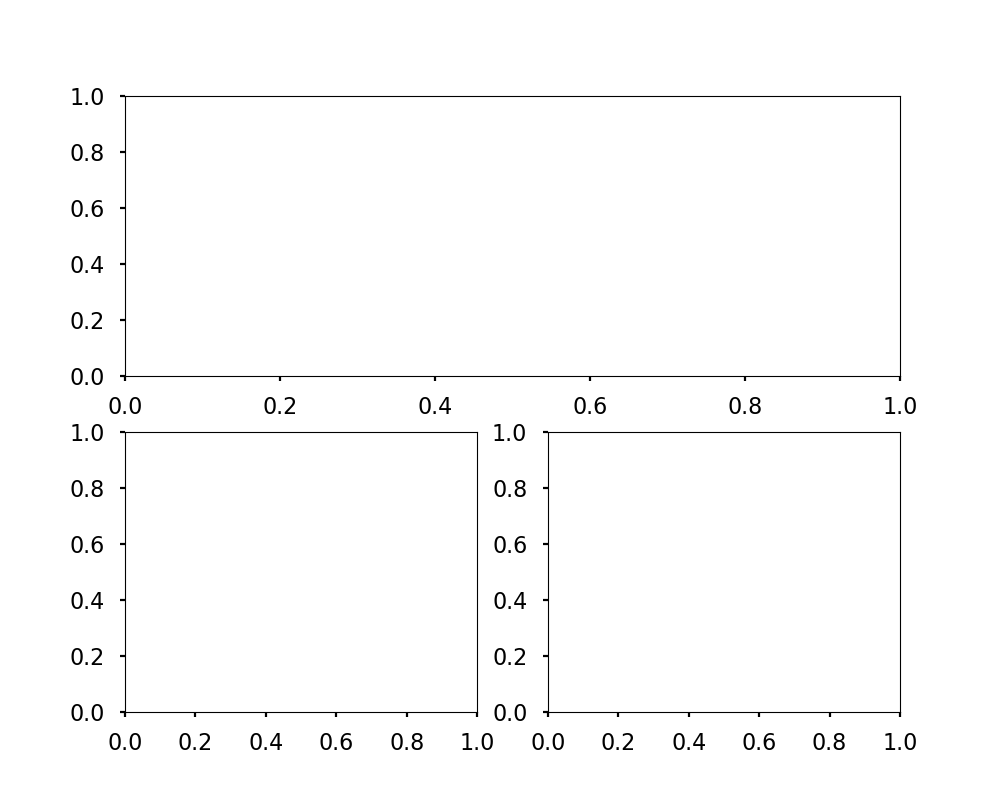
\includegraphics[width=\textwidth]{RQ13.png}
		\end{center}
		\column{0.5\textwidth}
		\vspace{-5mm}
		\begin{poll}
		\item
			\begin{pythoncode}
				ax1 = f.add_subplot(222)
				ax2 = f.add_subplot(221)
				ax3 = f.add_subplot(212)
			\end{pythoncode}

		\item
			\begin{pythoncode}
				ax1 = f.add_subplot(223)
				ax2 = f.add_subplot(221)
				ax3 = f.add_subplot(122)
			\end{pythoncode}

		\item
			\begin{pythoncode}
				ax1 = f.add_subplot(224)
				ax2 = f.add_subplot(223)
				ax3 = f.add_subplot(211)
			\end{pythoncode}

		\item
			\begin{pythoncode}
				ax1 = f.add_subplot(213)
				ax2 = f.add_subplot(211)
				ax3 = f.add_subplot(222)
			\end{pythoncode}
		\end{poll}
		\exsol{C}
	\end{columns}
\end{frame}

\begin{frame}{A Classy Arcade}
	\begin{itemize}
		\item We've been using \pyi{arcade} throughout the semester, but not to its full potential
		\item Like Matplotlib, Arcade is comprised of multiple classes that define specific objects
		\item We can inherit from those objects and then make small changes to get large amounts of functionality with relatively little effort!
	\end{itemize}
\end{frame}

\begin{frame}{Window to the Future}
	\begin{itemize}
		\item The primary class we can inherit from and use is \pyi{arcade.Window}
			\begin{itemize}
				\item The same class that was being formed when you used to call \pyi{arcade.open_window()}
			\end{itemize}
		\item The window class has a huge amount of predefined methods that we can override to provide almost any sort of flexibility
			\begin{itemize}
				\item \pyi{on_draw} for basic drawing
				\item \pyi{on_update} for animation
				\item Methods to get keyboard input
				\item Methods to get location and input from the mouse
				\item Methods to control what happens if the window is resized
				\item etc
			\end{itemize}
	\end{itemize}
\end{frame}

\begin{frame}[fragile]{Same Game, New Tricks}
	\begin{columns}[t]
		\column{0.5\textwidth}
		\begin{block}{Previously\ldots}
			\footnotesize
			\begin{pythoncode}
				import arcade

				arcade.open_window(
								500,
								500,
								'Hi')

				arcade.start_render()
				arcade.draw_circle_filled()
				arcade.finish_render()

				arcade.run()

			\end{pythoncode}
		\end{block}
		\column{0.5\textwidth}
		\begin{block}{Now\ldots}
			\footnotesize
			\begin{pythoncode}
				import arcade as arc

				class MyPicture(arc.Window):
					def __init__(self):
						arc.Window.__init__()
						arc.run()
			\end{pythoncode}
		\end{block}

		\pause
		\begin{itemize}
			\item So initially this is just organizing code
			\item But inheriting from the \pyi{arcade.Window} class gives us \alert{many} more options.
		\end{itemize}
	\end{columns}
\end{frame}

\begin{frame}[fragile]{On Draw!}
	\begin{itemize}
		\item We can override or redefine the \pyi{on_draw} method to specify what should happen whenever the window needs to draw something!
		\item Generally where you will put all of your \pyi{start_render} and \pyi{draw} commands
		\item You won't need to call the method yourself! The class knows what to do!
	\end{itemize}
	\begin{pythoncode}
		def on_draw(self):
			arcade.start_render()
			arcade.draw_circle_filled(
									200,
									200,
									100,
									arcade.color.YELLOW)
	\end{pythoncode}
	
\end{frame}

\begin{frame}[fragile]{On Update!}
	\begin{itemize}
		\item Can override the \pyi{on_update} method to control what happens when the window tries to update itself (usually about 60 times a second)
		\item Generally where animation controls should go
		\item Again, you won't need to call this method manually!
	\end{itemize}
	\medskip
	\begin{pythoncode}
		def on_update(self, dt):
			self.x += 1 # Assuming some circle uses self.x
			# Any other animation code you need to update
	\end{pythoncode}
\end{frame}

\begin{frame}[fragile]{On Key Press!}
	\begin{itemize}
		\item Override \pyi{on_key_press} to handle what should happen when any key is initially pressed
		\item \pyi{on_key_release} also exists if you want different functionality for that
		\item Takes two inputs: the key (as an integer code) and a modifier
		\item Can use the \pyi{arcade.key.<some key>} to easily look up the integer codes
	\end{itemize}
	\medskip
	\begin{pythoncode}
		def on_key_press(self, key, modifier):
			if key == arcade.key.Q:
				arcade.close_window()
	\end{pythoncode}
\end{frame}

\begin{frame}[fragile]{On Mouse Press!}
	\begin{itemize}
		\item Override \pyi{on_mouse_press} to handle anything that should happen when any mouse button is clicked
		\item Also options for release, drag, motion, etc
		\item \pyi{on_mouse_press} takes 4 arguments: x,y,button, and modifier
		\item Button codes are available from \pyi{arcade.MOUSE_<something>}
	\end{itemize}
	\medskip
	\begin{pythoncode}
		def on_mouse_press(self, x, y, button, modifier):
			if button == arcade.MOUSE_BUTTON_LEFT:
				print('Click!')
	\end{pythoncode}
	
\end{frame}








\end{document}

